% Quotation page (GPS item 4, one page). The author's drawing (front/quote.png, flattened onto white)
% fills the page: its 3160 x 4096 shape matches letter paper, so only a hair is cropped top and bottom.
% The quote sits in the drawing's blank band, about 35-58% of the way down and across the left three
% quarters (measured from the image). The page number stays where it is on every page (GPS); a small
% white patch keeps it legible over the drawing. Needs two runs (remember picture).
\clearpage
\thispagestyle{plain}
\addcontentsline{toc}{chapter}{Quotation}
\begin{tikzpicture}[remember picture, overlay]
\node[inner sep=0] (art) at (current page.center) {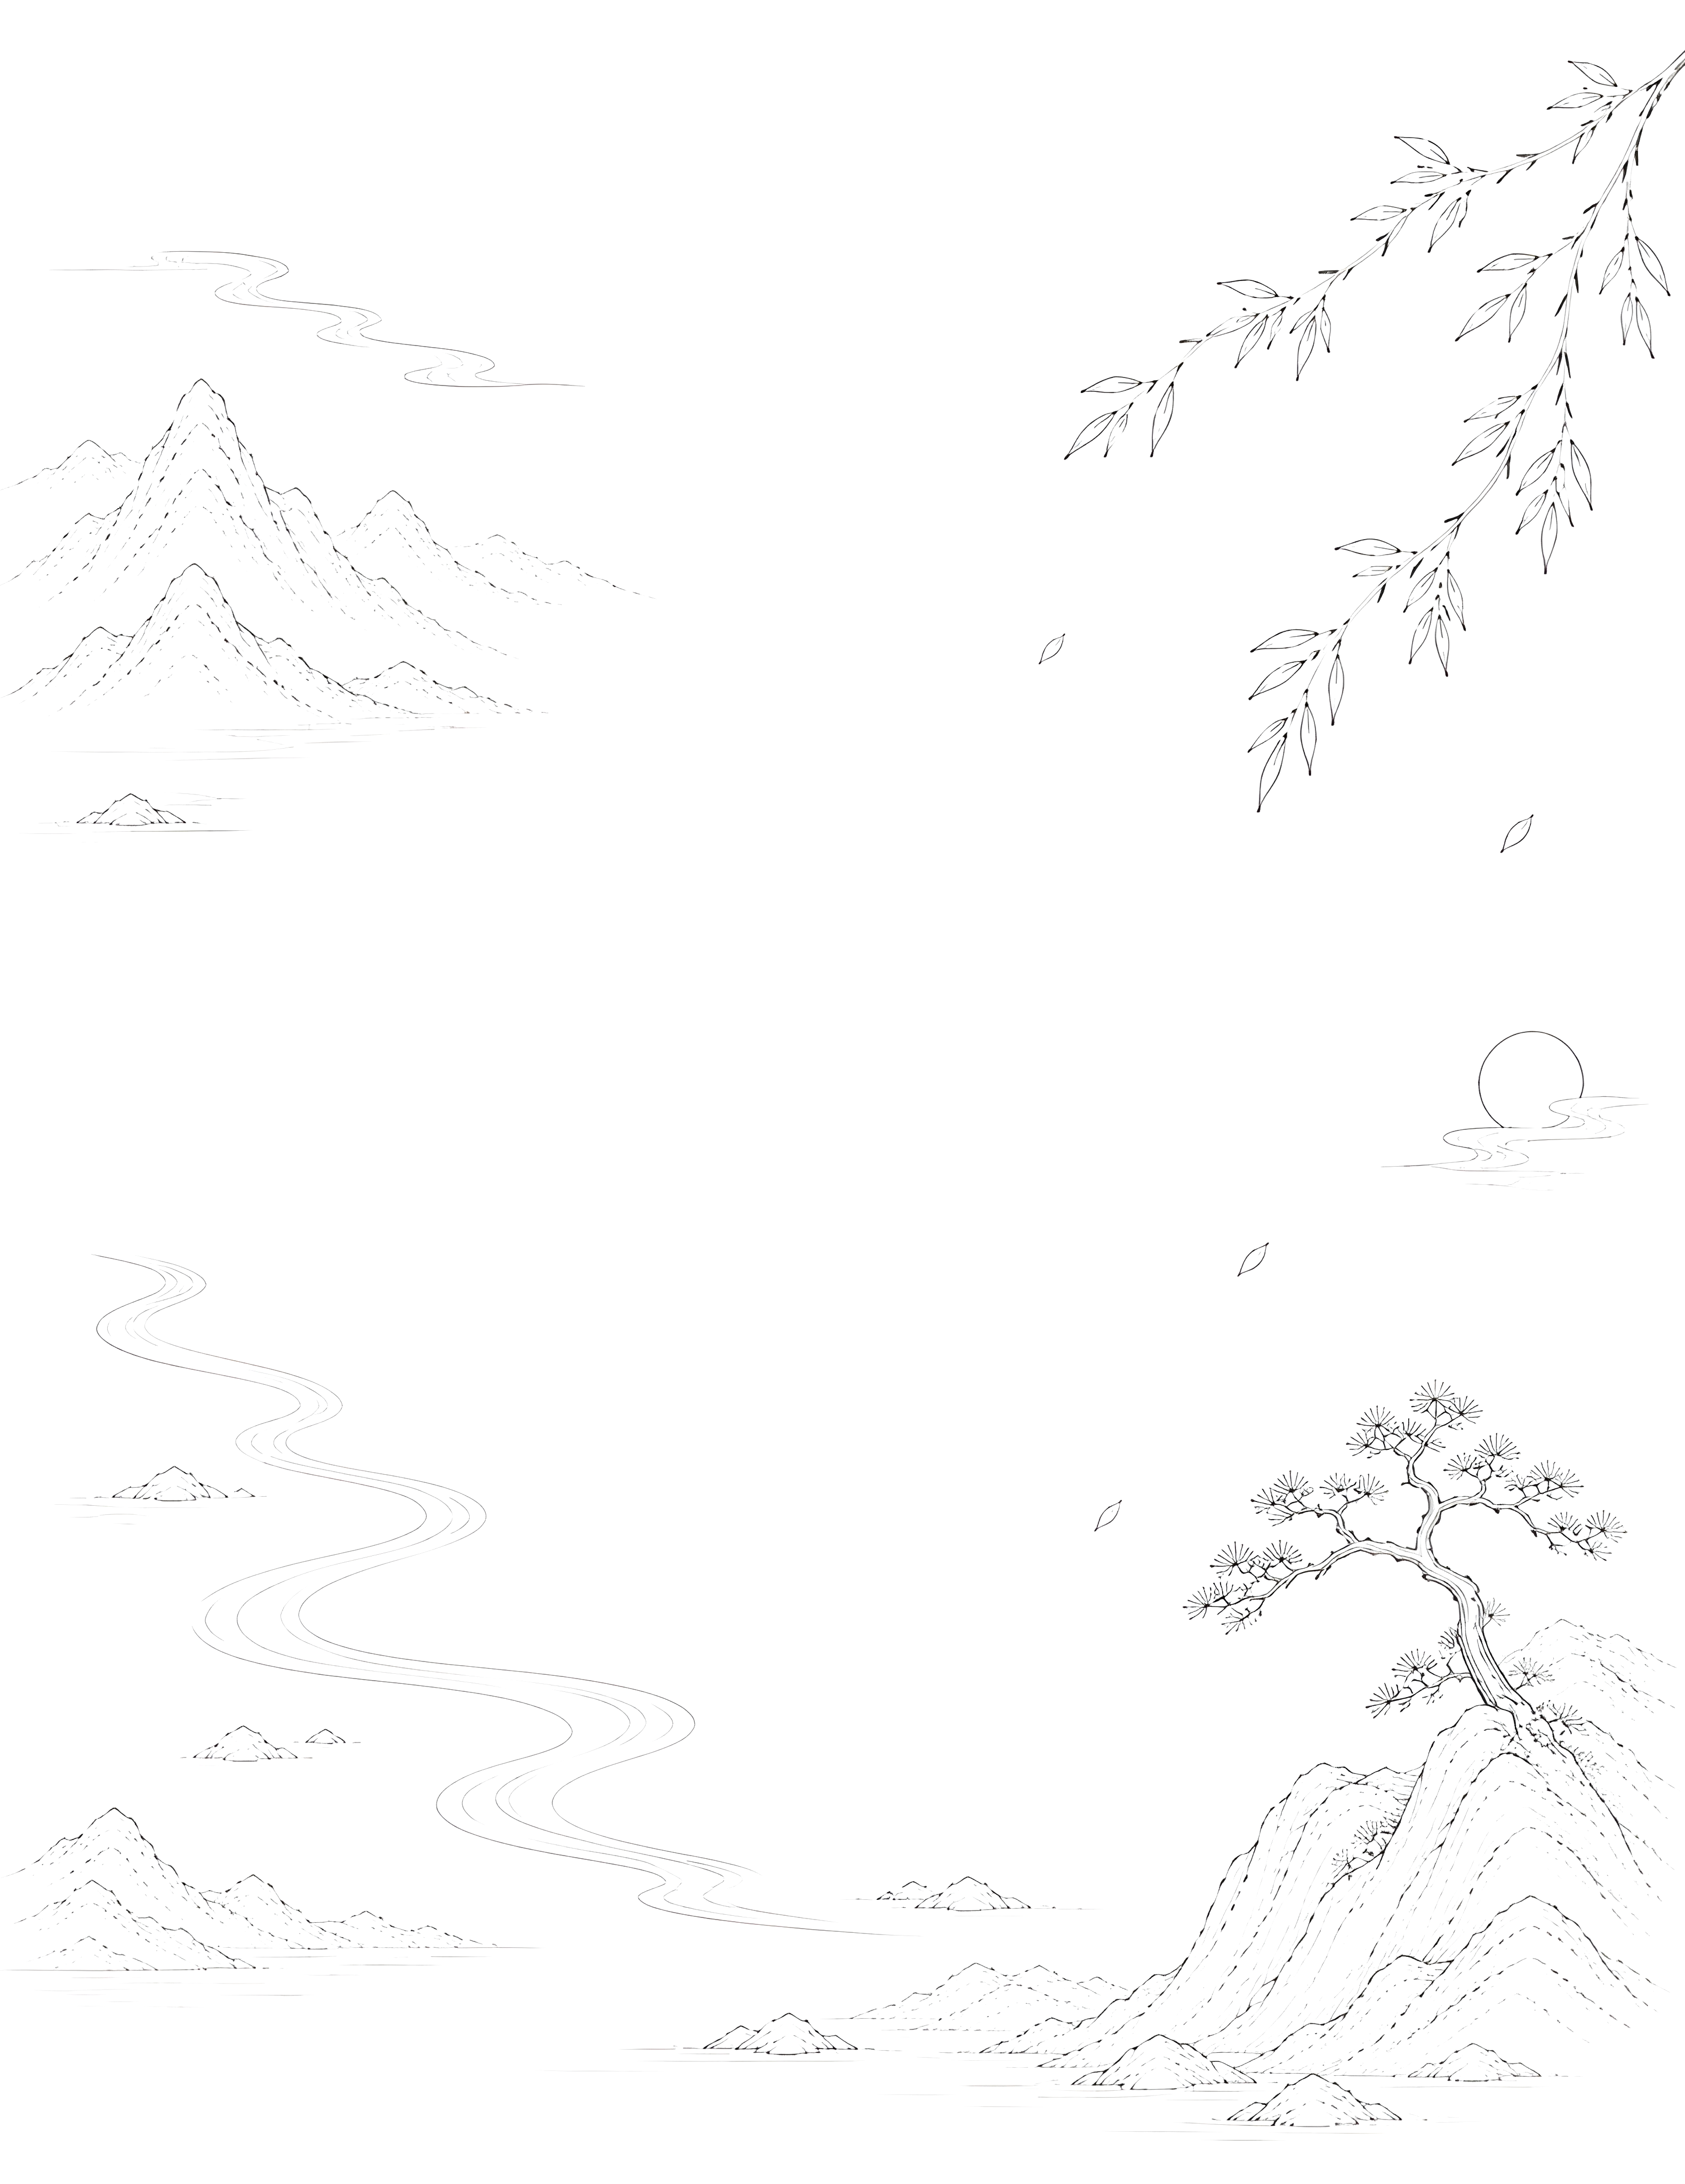
\includegraphics[width=\paperwidth]{front/quote.png}};
\begin{scope}[shift={(art.south west)}, x={(\paperwidth,0)}, y={(0,1.2962\paperwidth)}]
\node[align=center, font=\linespread{1}\selectfont] at (0.42, 0.535) {%
  \textit{The Tao that can be told}\\
  \textit{is not the eternal Tao.}\\
  \textit{The name that can be named}\\
  \textit{is not the eternal name.}\\[8pt]
  {\footnotesize Laozi, \textit{Tao Te Ching}, chapter 1}\\
  {\footnotesize trans.\ Gia-fu Feng and Jane English}};
\end{scope}
% Page-number position measured from the built PDF: centred 288pt from the left, 82pt from the bottom.
\node[fill=white, rounded corners=3pt, minimum width=36pt, minimum height=20pt]
  at ([xshift=288pt, yshift=82pt]current page.south west) {};
\end{tikzpicture}%
\null
